% Created by tikzDevice version 0.12.6 on 2024-01-05 10:48:34
% !TEX encoding = UTF-8 Unicode
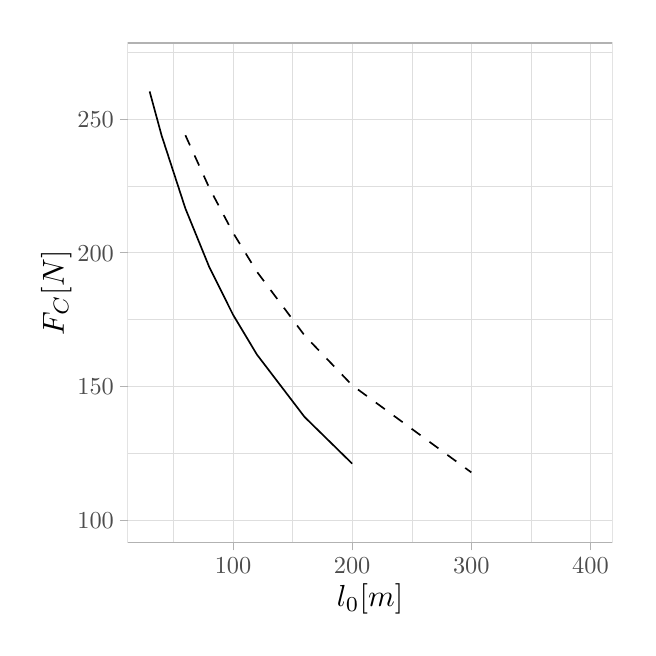
\begin{tikzpicture}[x=1pt,y=1pt]
\definecolor{fillColor}{RGB}{255,255,255}
\path[use as bounding box,fill=fillColor,fill opacity=0.00] (0,0) rectangle (216.81,216.81);
\begin{scope}
\path[clip] (  0.00,  0.00) rectangle (216.81,216.81);
\definecolor{drawColor}{RGB}{255,255,255}
\definecolor{fillColor}{RGB}{255,255,255}

\path[draw=drawColor,line width= 0.6pt,line join=round,line cap=round,fill=fillColor] (  0.00,  0.00) rectangle (216.81,216.81);
\end{scope}
\begin{scope}
\path[clip] ( 36.11, 30.69) rectangle (211.31,211.31);
\definecolor{fillColor}{RGB}{255,255,255}

\path[fill=fillColor] ( 36.11, 30.69) rectangle (211.31,211.31);
\definecolor{drawColor}{gray}{0.87}

\path[draw=drawColor,line width= 0.1pt,line join=round] ( 36.11, 63.04) --
	(211.31, 63.04);

\path[draw=drawColor,line width= 0.1pt,line join=round] ( 36.11,111.34) --
	(211.31,111.34);

\path[draw=drawColor,line width= 0.1pt,line join=round] ( 36.11,159.63) --
	(211.31,159.63);

\path[draw=drawColor,line width= 0.1pt,line join=round] ( 36.11,207.93) --
	(211.31,207.93);

\path[draw=drawColor,line width= 0.1pt,line join=round] ( 52.68, 30.69) --
	( 52.68,211.31);

\path[draw=drawColor,line width= 0.1pt,line join=round] ( 95.73, 30.69) --
	( 95.73,211.31);

\path[draw=drawColor,line width= 0.1pt,line join=round] (138.78, 30.69) --
	(138.78,211.31);

\path[draw=drawColor,line width= 0.1pt,line join=round] (181.82, 30.69) --
	(181.82,211.31);

\path[draw=drawColor,line width= 0.3pt,line join=round] ( 36.11, 38.90) --
	(211.31, 38.90);

\path[draw=drawColor,line width= 0.3pt,line join=round] ( 36.11, 87.19) --
	(211.31, 87.19);

\path[draw=drawColor,line width= 0.3pt,line join=round] ( 36.11,135.49) --
	(211.31,135.49);

\path[draw=drawColor,line width= 0.3pt,line join=round] ( 36.11,183.78) --
	(211.31,183.78);

\path[draw=drawColor,line width= 0.3pt,line join=round] ( 74.21, 30.69) --
	( 74.21,211.31);

\path[draw=drawColor,line width= 0.3pt,line join=round] (117.25, 30.69) --
	(117.25,211.31);

\path[draw=drawColor,line width= 0.3pt,line join=round] (160.30, 30.69) --
	(160.30,211.31);

\path[draw=drawColor,line width= 0.3pt,line join=round] (203.35, 30.69) --
	(203.35,211.31);
\definecolor{drawColor}{RGB}{0,0,0}

\path[draw=drawColor,line width= 0.6pt,line join=round] ( 44.07,193.76) --
	( 48.38,177.90) --
	( 56.99,151.47) --
	( 65.60,130.35) --
	( 74.21,113.08) --
	( 82.82, 98.71) --
	(100.04, 76.15) --
	(117.25, 59.28);

\path[draw=drawColor,line width= 0.6pt,dash pattern=on 4pt off 4pt ,line join=round] ( 56.99,177.93) --
	( 65.60,158.97) --
	( 74.21,142.71) --
	( 82.82,128.65) --
	(100.04,105.61) --
	(117.25, 87.59) --
	(160.30, 56.11);
\definecolor{drawColor}{gray}{0.70}

\path[draw=drawColor,line width= 0.6pt,line join=round,line cap=round] ( 36.11, 30.69) rectangle (211.31,211.31);
\end{scope}
\begin{scope}
\path[clip] (  0.00,  0.00) rectangle (216.81,216.81);
\definecolor{drawColor}{gray}{0.30}

\node[text=drawColor,anchor=base east,inner sep=0pt, outer sep=0pt, scale=  0.88] at ( 31.16, 35.87) {100};

\node[text=drawColor,anchor=base east,inner sep=0pt, outer sep=0pt, scale=  0.88] at ( 31.16, 84.16) {150};

\node[text=drawColor,anchor=base east,inner sep=0pt, outer sep=0pt, scale=  0.88] at ( 31.16,132.46) {200};

\node[text=drawColor,anchor=base east,inner sep=0pt, outer sep=0pt, scale=  0.88] at ( 31.16,180.75) {250};
\end{scope}
\begin{scope}
\path[clip] (  0.00,  0.00) rectangle (216.81,216.81);
\definecolor{drawColor}{gray}{0.70}

\path[draw=drawColor,line width= 0.3pt,line join=round] ( 33.36, 38.90) --
	( 36.11, 38.90);

\path[draw=drawColor,line width= 0.3pt,line join=round] ( 33.36, 87.19) --
	( 36.11, 87.19);

\path[draw=drawColor,line width= 0.3pt,line join=round] ( 33.36,135.49) --
	( 36.11,135.49);

\path[draw=drawColor,line width= 0.3pt,line join=round] ( 33.36,183.78) --
	( 36.11,183.78);
\end{scope}
\begin{scope}
\path[clip] (  0.00,  0.00) rectangle (216.81,216.81);
\definecolor{drawColor}{gray}{0.70}

\path[draw=drawColor,line width= 0.3pt,line join=round] ( 74.21, 27.94) --
	( 74.21, 30.69);

\path[draw=drawColor,line width= 0.3pt,line join=round] (117.25, 27.94) --
	(117.25, 30.69);

\path[draw=drawColor,line width= 0.3pt,line join=round] (160.30, 27.94) --
	(160.30, 30.69);

\path[draw=drawColor,line width= 0.3pt,line join=round] (203.35, 27.94) --
	(203.35, 30.69);
\end{scope}
\begin{scope}
\path[clip] (  0.00,  0.00) rectangle (216.81,216.81);
\definecolor{drawColor}{gray}{0.30}

\node[text=drawColor,anchor=base,inner sep=0pt, outer sep=0pt, scale=  0.88] at ( 74.21, 19.68) {100};

\node[text=drawColor,anchor=base,inner sep=0pt, outer sep=0pt, scale=  0.88] at (117.25, 19.68) {200};

\node[text=drawColor,anchor=base,inner sep=0pt, outer sep=0pt, scale=  0.88] at (160.30, 19.68) {300};

\node[text=drawColor,anchor=base,inner sep=0pt, outer sep=0pt, scale=  0.88] at (203.35, 19.68) {400};
\end{scope}
\begin{scope}
\path[clip] (  0.00,  0.00) rectangle (216.81,216.81);
\definecolor{drawColor}{RGB}{0,0,0}

\node[text=drawColor,anchor=base,inner sep=0pt, outer sep=0pt, scale=  1.10] at (123.71,  7.64) {$l_0 [m]$};
\end{scope}
\begin{scope}
\path[clip] (  0.00,  0.00) rectangle (216.81,216.81);
\definecolor{drawColor}{RGB}{0,0,0}

\node[text=drawColor,rotate= 90.00,anchor=base,inner sep=0pt, outer sep=0pt, scale=  1.10] at ( 13.08,121.00) {$F_C [N]$};
\end{scope}
\end{tikzpicture}
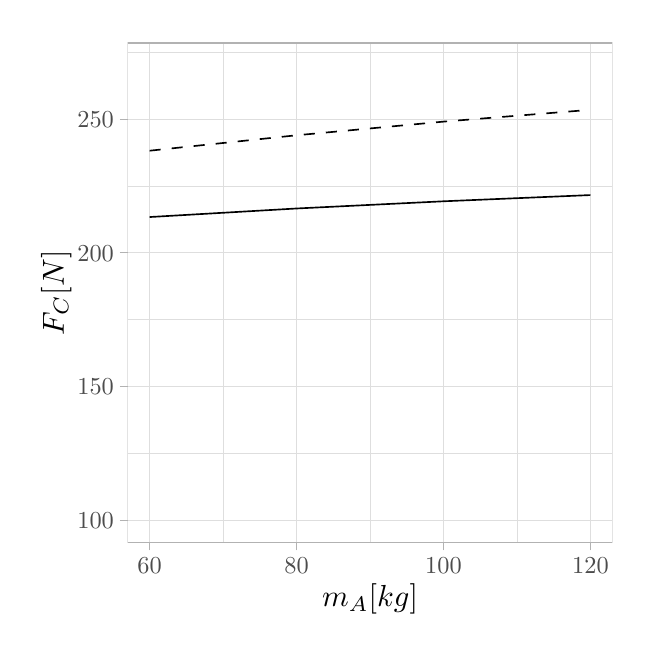
\begin{tikzpicture}[x=1pt,y=1pt]
\definecolor{fillColor}{RGB}{255,255,255}
\path[use as bounding box,fill=fillColor,fill opacity=0.00] (0,0) rectangle (216.81,216.81);
\begin{scope}
\path[clip] (  0.00,  0.00) rectangle (216.81,216.81);
\definecolor{drawColor}{RGB}{255,255,255}
\definecolor{fillColor}{RGB}{255,255,255}

\path[draw=drawColor,line width= 0.6pt,line join=round,line cap=round,fill=fillColor] (  0.00,  0.00) rectangle (216.81,216.81);
\end{scope}
\begin{scope}
\path[clip] ( 36.11, 30.69) rectangle (211.31,211.31);
\definecolor{fillColor}{RGB}{255,255,255}

\path[fill=fillColor] ( 36.11, 30.69) rectangle (211.31,211.31);
\definecolor{drawColor}{gray}{0.87}

\path[draw=drawColor,line width= 0.1pt,line join=round] ( 36.11, 63.04) --
	(211.31, 63.04);

\path[draw=drawColor,line width= 0.1pt,line join=round] ( 36.11,111.34) --
	(211.31,111.34);

\path[draw=drawColor,line width= 0.1pt,line join=round] ( 36.11,159.63) --
	(211.31,159.63);

\path[draw=drawColor,line width= 0.1pt,line join=round] ( 36.11,207.93) --
	(211.31,207.93);

\path[draw=drawColor,line width= 0.1pt,line join=round] ( 70.62, 30.69) --
	( 70.62,211.31);

\path[draw=drawColor,line width= 0.1pt,line join=round] (123.71, 30.69) --
	(123.71,211.31);

\path[draw=drawColor,line width= 0.1pt,line join=round] (176.80, 30.69) --
	(176.80,211.31);

\path[draw=drawColor,line width= 0.3pt,line join=round] ( 36.11, 38.90) --
	(211.31, 38.90);

\path[draw=drawColor,line width= 0.3pt,line join=round] ( 36.11, 87.19) --
	(211.31, 87.19);

\path[draw=drawColor,line width= 0.3pt,line join=round] ( 36.11,135.49) --
	(211.31,135.49);

\path[draw=drawColor,line width= 0.3pt,line join=round] ( 36.11,183.78) --
	(211.31,183.78);

\path[draw=drawColor,line width= 0.3pt,line join=round] ( 44.07, 30.69) --
	( 44.07,211.31);

\path[draw=drawColor,line width= 0.3pt,line join=round] ( 97.17, 30.69) --
	( 97.17,211.31);

\path[draw=drawColor,line width= 0.3pt,line join=round] (150.26, 30.69) --
	(150.26,211.31);

\path[draw=drawColor,line width= 0.3pt,line join=round] (203.35, 30.69) --
	(203.35,211.31);
\definecolor{drawColor}{RGB}{0,0,0}

\path[draw=drawColor,line width= 0.6pt,line join=round] ( 44.07,148.38) --
	( 97.17,151.47) --
	(150.26,154.07) --
	(203.35,156.32);

\path[draw=drawColor,line width= 0.6pt,dash pattern=on 4pt off 4pt ,line join=round] ( 44.07,172.35) --
	( 97.17,177.93) --
	(150.26,182.86) --
	(203.35,187.13);
\definecolor{drawColor}{gray}{0.70}

\path[draw=drawColor,line width= 0.6pt,line join=round,line cap=round] ( 36.11, 30.69) rectangle (211.31,211.31);
\end{scope}
\begin{scope}
\path[clip] (  0.00,  0.00) rectangle (216.81,216.81);
\definecolor{drawColor}{gray}{0.30}

\node[text=drawColor,anchor=base east,inner sep=0pt, outer sep=0pt, scale=  0.88] at ( 31.16, 35.87) {100};

\node[text=drawColor,anchor=base east,inner sep=0pt, outer sep=0pt, scale=  0.88] at ( 31.16, 84.16) {150};

\node[text=drawColor,anchor=base east,inner sep=0pt, outer sep=0pt, scale=  0.88] at ( 31.16,132.46) {200};

\node[text=drawColor,anchor=base east,inner sep=0pt, outer sep=0pt, scale=  0.88] at ( 31.16,180.75) {250};
\end{scope}
\begin{scope}
\path[clip] (  0.00,  0.00) rectangle (216.81,216.81);
\definecolor{drawColor}{gray}{0.70}

\path[draw=drawColor,line width= 0.3pt,line join=round] ( 33.36, 38.90) --
	( 36.11, 38.90);

\path[draw=drawColor,line width= 0.3pt,line join=round] ( 33.36, 87.19) --
	( 36.11, 87.19);

\path[draw=drawColor,line width= 0.3pt,line join=round] ( 33.36,135.49) --
	( 36.11,135.49);

\path[draw=drawColor,line width= 0.3pt,line join=round] ( 33.36,183.78) --
	( 36.11,183.78);
\end{scope}
\begin{scope}
\path[clip] (  0.00,  0.00) rectangle (216.81,216.81);
\definecolor{drawColor}{gray}{0.70}

\path[draw=drawColor,line width= 0.3pt,line join=round] ( 44.07, 27.94) --
	( 44.07, 30.69);

\path[draw=drawColor,line width= 0.3pt,line join=round] ( 97.17, 27.94) --
	( 97.17, 30.69);

\path[draw=drawColor,line width= 0.3pt,line join=round] (150.26, 27.94) --
	(150.26, 30.69);

\path[draw=drawColor,line width= 0.3pt,line join=round] (203.35, 27.94) --
	(203.35, 30.69);
\end{scope}
\begin{scope}
\path[clip] (  0.00,  0.00) rectangle (216.81,216.81);
\definecolor{drawColor}{gray}{0.30}

\node[text=drawColor,anchor=base,inner sep=0pt, outer sep=0pt, scale=  0.88] at ( 44.07, 19.68) {60};

\node[text=drawColor,anchor=base,inner sep=0pt, outer sep=0pt, scale=  0.88] at ( 97.17, 19.68) {80};

\node[text=drawColor,anchor=base,inner sep=0pt, outer sep=0pt, scale=  0.88] at (150.26, 19.68) {100};

\node[text=drawColor,anchor=base,inner sep=0pt, outer sep=0pt, scale=  0.88] at (203.35, 19.68) {120};
\end{scope}
\begin{scope}
\path[clip] (  0.00,  0.00) rectangle (216.81,216.81);
\definecolor{drawColor}{RGB}{0,0,0}

\node[text=drawColor,anchor=base,inner sep=0pt, outer sep=0pt, scale=  1.10] at (123.71,  7.64) {$m_A [kg]$};
\end{scope}
\begin{scope}
\path[clip] (  0.00,  0.00) rectangle (216.81,216.81);
\definecolor{drawColor}{RGB}{0,0,0}

\node[text=drawColor,rotate= 90.00,anchor=base,inner sep=0pt, outer sep=0pt, scale=  1.10] at ( 13.08,121.00) {$F_C [N]$};
\end{scope}
\end{tikzpicture}
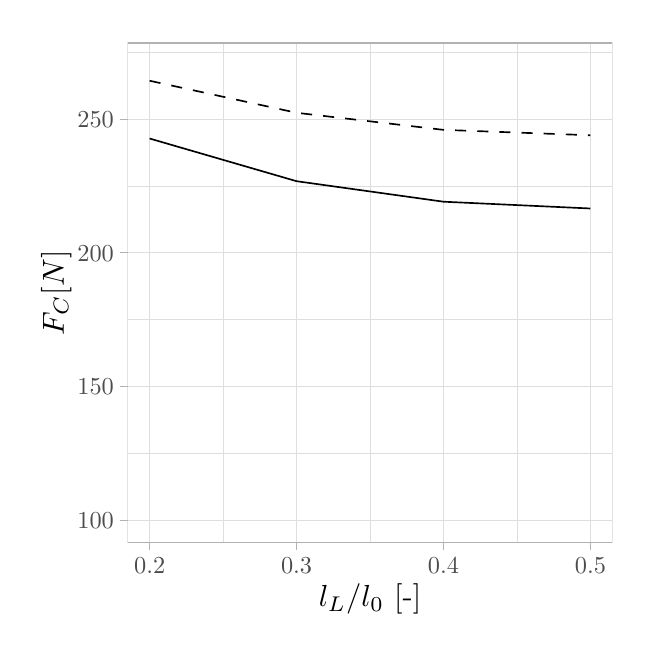
\begin{tikzpicture}[x=1pt,y=1pt]
\definecolor{fillColor}{RGB}{255,255,255}
\path[use as bounding box,fill=fillColor,fill opacity=0.00] (0,0) rectangle (216.81,216.81);
\begin{scope}
\path[clip] (  0.00,  0.00) rectangle (216.81,216.81);
\definecolor{drawColor}{RGB}{255,255,255}
\definecolor{fillColor}{RGB}{255,255,255}

\path[draw=drawColor,line width= 0.6pt,line join=round,line cap=round,fill=fillColor] (  0.00,  0.00) rectangle (216.81,216.81);
\end{scope}
\begin{scope}
\path[clip] ( 36.11, 30.69) rectangle (211.31,211.31);
\definecolor{fillColor}{RGB}{255,255,255}

\path[fill=fillColor] ( 36.11, 30.69) rectangle (211.31,211.31);
\definecolor{drawColor}{gray}{0.87}

\path[draw=drawColor,line width= 0.1pt,line join=round] ( 36.11, 63.04) --
	(211.31, 63.04);

\path[draw=drawColor,line width= 0.1pt,line join=round] ( 36.11,111.34) --
	(211.31,111.34);

\path[draw=drawColor,line width= 0.1pt,line join=round] ( 36.11,159.63) --
	(211.31,159.63);

\path[draw=drawColor,line width= 0.1pt,line join=round] ( 36.11,207.93) --
	(211.31,207.93);

\path[draw=drawColor,line width= 0.1pt,line join=round] ( 70.62, 30.69) --
	( 70.62,211.31);

\path[draw=drawColor,line width= 0.1pt,line join=round] (123.71, 30.69) --
	(123.71,211.31);

\path[draw=drawColor,line width= 0.1pt,line join=round] (176.80, 30.69) --
	(176.80,211.31);

\path[draw=drawColor,line width= 0.3pt,line join=round] ( 36.11, 38.90) --
	(211.31, 38.90);

\path[draw=drawColor,line width= 0.3pt,line join=round] ( 36.11, 87.19) --
	(211.31, 87.19);

\path[draw=drawColor,line width= 0.3pt,line join=round] ( 36.11,135.49) --
	(211.31,135.49);

\path[draw=drawColor,line width= 0.3pt,line join=round] ( 36.11,183.78) --
	(211.31,183.78);

\path[draw=drawColor,line width= 0.3pt,line join=round] ( 44.07, 30.69) --
	( 44.07,211.31);

\path[draw=drawColor,line width= 0.3pt,line join=round] ( 97.17, 30.69) --
	( 97.17,211.31);

\path[draw=drawColor,line width= 0.3pt,line join=round] (150.26, 30.69) --
	(150.26,211.31);

\path[draw=drawColor,line width= 0.3pt,line join=round] (203.35, 30.69) --
	(203.35,211.31);
\definecolor{drawColor}{RGB}{0,0,0}

\path[draw=drawColor,line width= 0.6pt,line join=round] ( 44.07,176.75) --
	( 97.17,161.33) --
	(150.26,153.92) --
	(203.35,151.47);

\path[draw=drawColor,line width= 0.6pt,dash pattern=on 4pt off 4pt ,line join=round] ( 44.07,197.63) --
	( 97.17,186.05) --
	(150.26,179.88) --
	(203.35,177.93);
\definecolor{drawColor}{gray}{0.70}

\path[draw=drawColor,line width= 0.6pt,line join=round,line cap=round] ( 36.11, 30.69) rectangle (211.31,211.31);
\end{scope}
\begin{scope}
\path[clip] (  0.00,  0.00) rectangle (216.81,216.81);
\definecolor{drawColor}{gray}{0.30}

\node[text=drawColor,anchor=base east,inner sep=0pt, outer sep=0pt, scale=  0.88] at ( 31.16, 35.87) {100};

\node[text=drawColor,anchor=base east,inner sep=0pt, outer sep=0pt, scale=  0.88] at ( 31.16, 84.16) {150};

\node[text=drawColor,anchor=base east,inner sep=0pt, outer sep=0pt, scale=  0.88] at ( 31.16,132.46) {200};

\node[text=drawColor,anchor=base east,inner sep=0pt, outer sep=0pt, scale=  0.88] at ( 31.16,180.75) {250};
\end{scope}
\begin{scope}
\path[clip] (  0.00,  0.00) rectangle (216.81,216.81);
\definecolor{drawColor}{gray}{0.70}

\path[draw=drawColor,line width= 0.3pt,line join=round] ( 33.36, 38.90) --
	( 36.11, 38.90);

\path[draw=drawColor,line width= 0.3pt,line join=round] ( 33.36, 87.19) --
	( 36.11, 87.19);

\path[draw=drawColor,line width= 0.3pt,line join=round] ( 33.36,135.49) --
	( 36.11,135.49);

\path[draw=drawColor,line width= 0.3pt,line join=round] ( 33.36,183.78) --
	( 36.11,183.78);
\end{scope}
\begin{scope}
\path[clip] (  0.00,  0.00) rectangle (216.81,216.81);
\definecolor{drawColor}{gray}{0.70}

\path[draw=drawColor,line width= 0.3pt,line join=round] ( 44.07, 27.94) --
	( 44.07, 30.69);

\path[draw=drawColor,line width= 0.3pt,line join=round] ( 97.17, 27.94) --
	( 97.17, 30.69);

\path[draw=drawColor,line width= 0.3pt,line join=round] (150.26, 27.94) --
	(150.26, 30.69);

\path[draw=drawColor,line width= 0.3pt,line join=round] (203.35, 27.94) --
	(203.35, 30.69);
\end{scope}
\begin{scope}
\path[clip] (  0.00,  0.00) rectangle (216.81,216.81);
\definecolor{drawColor}{gray}{0.30}

\node[text=drawColor,anchor=base,inner sep=0pt, outer sep=0pt, scale=  0.88] at ( 44.07, 19.68) {0.2};

\node[text=drawColor,anchor=base,inner sep=0pt, outer sep=0pt, scale=  0.88] at ( 97.17, 19.68) {0.3};

\node[text=drawColor,anchor=base,inner sep=0pt, outer sep=0pt, scale=  0.88] at (150.26, 19.68) {0.4};

\node[text=drawColor,anchor=base,inner sep=0pt, outer sep=0pt, scale=  0.88] at (203.35, 19.68) {0.5};
\end{scope}
\begin{scope}
\path[clip] (  0.00,  0.00) rectangle (216.81,216.81);
\definecolor{drawColor}{RGB}{0,0,0}

\node[text=drawColor,anchor=base,inner sep=0pt, outer sep=0pt, scale=  1.10] at (123.71,  7.64) {$l_L/l_0$ [-]};
\end{scope}
\begin{scope}
\path[clip] (  0.00,  0.00) rectangle (216.81,216.81);
\definecolor{drawColor}{RGB}{0,0,0}

\node[text=drawColor,rotate= 90.00,anchor=base,inner sep=0pt, outer sep=0pt, scale=  1.10] at ( 13.08,121.00) {$F_C [N]$};
\end{scope}
\end{tikzpicture}
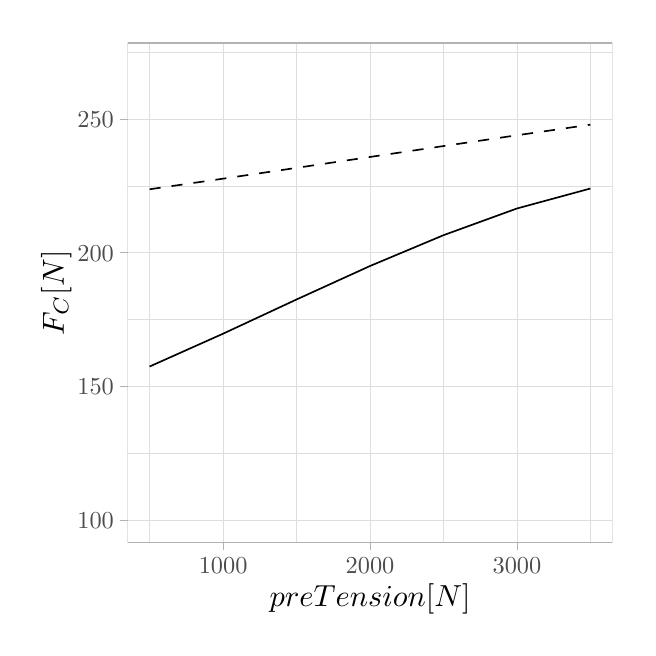
\begin{tikzpicture}[x=1pt,y=1pt]
\definecolor{fillColor}{RGB}{255,255,255}
\path[use as bounding box,fill=fillColor,fill opacity=0.00] (0,0) rectangle (216.81,216.81);
\begin{scope}
\path[clip] (  0.00,  0.00) rectangle (216.81,216.81);
\definecolor{drawColor}{RGB}{255,255,255}
\definecolor{fillColor}{RGB}{255,255,255}

\path[draw=drawColor,line width= 0.6pt,line join=round,line cap=round,fill=fillColor] (  0.00,  0.00) rectangle (216.81,216.81);
\end{scope}
\begin{scope}
\path[clip] ( 36.11, 30.69) rectangle (211.31,211.31);
\definecolor{fillColor}{RGB}{255,255,255}

\path[fill=fillColor] ( 36.11, 30.69) rectangle (211.31,211.31);
\definecolor{drawColor}{gray}{0.87}

\path[draw=drawColor,line width= 0.1pt,line join=round] ( 36.11, 63.04) --
	(211.31, 63.04);

\path[draw=drawColor,line width= 0.1pt,line join=round] ( 36.11,111.34) --
	(211.31,111.34);

\path[draw=drawColor,line width= 0.1pt,line join=round] ( 36.11,159.63) --
	(211.31,159.63);

\path[draw=drawColor,line width= 0.1pt,line join=round] ( 36.11,207.93) --
	(211.31,207.93);

\path[draw=drawColor,line width= 0.1pt,line join=round] ( 44.07, 30.69) --
	( 44.07,211.31);

\path[draw=drawColor,line width= 0.1pt,line join=round] ( 97.17, 30.69) --
	( 97.17,211.31);

\path[draw=drawColor,line width= 0.1pt,line join=round] (150.26, 30.69) --
	(150.26,211.31);

\path[draw=drawColor,line width= 0.1pt,line join=round] (203.35, 30.69) --
	(203.35,211.31);

\path[draw=drawColor,line width= 0.3pt,line join=round] ( 36.11, 38.90) --
	(211.31, 38.90);

\path[draw=drawColor,line width= 0.3pt,line join=round] ( 36.11, 87.19) --
	(211.31, 87.19);

\path[draw=drawColor,line width= 0.3pt,line join=round] ( 36.11,135.49) --
	(211.31,135.49);

\path[draw=drawColor,line width= 0.3pt,line join=round] ( 36.11,183.78) --
	(211.31,183.78);

\path[draw=drawColor,line width= 0.3pt,line join=round] ( 70.62, 30.69) --
	( 70.62,211.31);

\path[draw=drawColor,line width= 0.3pt,line join=round] (123.71, 30.69) --
	(123.71,211.31);

\path[draw=drawColor,line width= 0.3pt,line join=round] (176.80, 30.69) --
	(176.80,211.31);
\definecolor{drawColor}{RGB}{0,0,0}

\path[draw=drawColor,line width= 0.6pt,line join=round] ( 44.07, 94.37) --
	( 70.62,106.23) --
	( 97.17,118.60) --
	(123.71,130.69) --
	(150.26,141.82) --
	(176.80,151.47) --
	(203.35,158.69);

\path[draw=drawColor,line width= 0.6pt,dash pattern=on 4pt off 4pt ,line join=round] ( 44.07,158.41) --
	( 70.62,162.25) --
	( 97.17,166.15) --
	(123.71,170.09) --
	(150.26,174.03) --
	(176.80,177.93) --
	(203.35,181.76);
\definecolor{drawColor}{gray}{0.70}

\path[draw=drawColor,line width= 0.6pt,line join=round,line cap=round] ( 36.11, 30.69) rectangle (211.31,211.31);
\end{scope}
\begin{scope}
\path[clip] (  0.00,  0.00) rectangle (216.81,216.81);
\definecolor{drawColor}{gray}{0.30}

\node[text=drawColor,anchor=base east,inner sep=0pt, outer sep=0pt, scale=  0.88] at ( 31.16, 35.87) {100};

\node[text=drawColor,anchor=base east,inner sep=0pt, outer sep=0pt, scale=  0.88] at ( 31.16, 84.16) {150};

\node[text=drawColor,anchor=base east,inner sep=0pt, outer sep=0pt, scale=  0.88] at ( 31.16,132.46) {200};

\node[text=drawColor,anchor=base east,inner sep=0pt, outer sep=0pt, scale=  0.88] at ( 31.16,180.75) {250};
\end{scope}
\begin{scope}
\path[clip] (  0.00,  0.00) rectangle (216.81,216.81);
\definecolor{drawColor}{gray}{0.70}

\path[draw=drawColor,line width= 0.3pt,line join=round] ( 33.36, 38.90) --
	( 36.11, 38.90);

\path[draw=drawColor,line width= 0.3pt,line join=round] ( 33.36, 87.19) --
	( 36.11, 87.19);

\path[draw=drawColor,line width= 0.3pt,line join=round] ( 33.36,135.49) --
	( 36.11,135.49);

\path[draw=drawColor,line width= 0.3pt,line join=round] ( 33.36,183.78) --
	( 36.11,183.78);
\end{scope}
\begin{scope}
\path[clip] (  0.00,  0.00) rectangle (216.81,216.81);
\definecolor{drawColor}{gray}{0.70}

\path[draw=drawColor,line width= 0.3pt,line join=round] ( 70.62, 27.94) --
	( 70.62, 30.69);

\path[draw=drawColor,line width= 0.3pt,line join=round] (123.71, 27.94) --
	(123.71, 30.69);

\path[draw=drawColor,line width= 0.3pt,line join=round] (176.80, 27.94) --
	(176.80, 30.69);
\end{scope}
\begin{scope}
\path[clip] (  0.00,  0.00) rectangle (216.81,216.81);
\definecolor{drawColor}{gray}{0.30}

\node[text=drawColor,anchor=base,inner sep=0pt, outer sep=0pt, scale=  0.88] at ( 70.62, 19.68) {1000};

\node[text=drawColor,anchor=base,inner sep=0pt, outer sep=0pt, scale=  0.88] at (123.71, 19.68) {2000};

\node[text=drawColor,anchor=base,inner sep=0pt, outer sep=0pt, scale=  0.88] at (176.80, 19.68) {3000};
\end{scope}
\begin{scope}
\path[clip] (  0.00,  0.00) rectangle (216.81,216.81);
\definecolor{drawColor}{RGB}{0,0,0}

\node[text=drawColor,anchor=base,inner sep=0pt, outer sep=0pt, scale=  1.10] at (123.71,  7.64) {$preTension [N]$};
\end{scope}
\begin{scope}
\path[clip] (  0.00,  0.00) rectangle (216.81,216.81);
\definecolor{drawColor}{RGB}{0,0,0}

\node[text=drawColor,rotate= 90.00,anchor=base,inner sep=0pt, outer sep=0pt, scale=  1.10] at ( 13.08,121.00) {$F_C [N]$};
\end{scope}
\end{tikzpicture}
